Hier ist das ER Diagramm welches von unserer Datenbank durch Migrationen umgesetzt wurde.

\begin{figure}[H]
	\begin{center}
		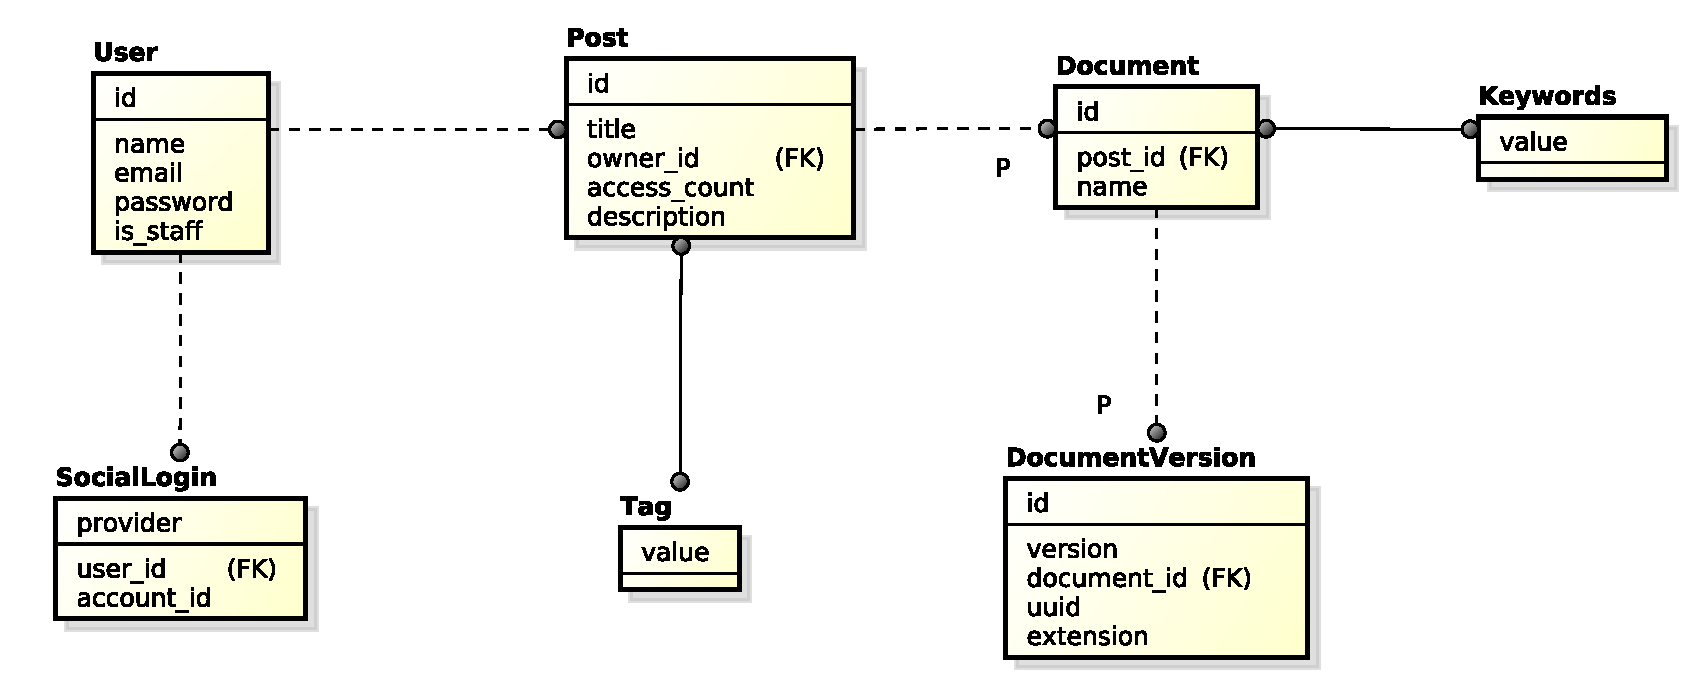
\includegraphics[width=\linewidth]{../Datenstruktur.pdf}
		\caption{ER Diagramm}
	\end{center}
\end{figure}

\section{Weiter Entwicklung}

Migrationen sind ein Weg um in Laravel Datenbank Strukturen umzusetzen

Hier ein Beispiel, welches die User Tabelle definiert.

\begin{lstlisting}[language={PHP}, caption="Migrations Beispiel"]
  class CreateUsersTable extends Migration
  {
      // Run the migrations.
      public function up()
      {
          Schema::create('users', function (Blueprint $table) {
              $table->increments('id');
              $table->string('name');
              $table->string('email')->unique();
              $table->string('password', 60);
              $table->rememberToken();
              $table->timestamps();
          });
      }

      // Reverse the migrations.
      public function down()
      {
          Schema::drop('users');
      }
  }
\end{lstlisting}

Eine Migration wird erstellt mittels \texttt{php artisan create:migration [name]} und ist dann unter dem Ordner \texttt{database/migrations} mit allen bisherigen Migrationen zu finden und zu editieren.
Um dann die Datenbank zu migrieren (Datenstruktur erstellen und nicht zu verwechseln mit dem Migrationsscript) wird \texttt{php artisan migrate}
Eine n\"ahere Dokumentation zu Migrations in Laravel sind in der \href{https://laravel.com/docs/5.2/migrations}{Offiziellen Dokumentation} zu finden
